\documentclass{article}
\usepackage{graphicx}
\usepackage{hyperref}
\usepackage[utf8]{inputenc}
\usepackage{lipsum}
\usepackage{courier} %% Sets font for listing as Courier.
\usepackage{listings, xcolor}
\usepackage{biblatex}
\usepackage{longtable}
\addbibresource{test.bib}

\lstset{
tabsize = 4, %% set tab space width
showstringspaces = false, %% prevent space marking in strings, string is defined as the text that is generally printed directly to the console
numbers = left, %% display line numbers on the left
commentstyle = \color{green}, %% set comment color
keywordstyle = \color{blue}, %% set keyword color
stringstyle = \color{red}, %% set string color
rulecolor = \color{black}, %% set frame color to avoid being affected by text color
basicstyle = \ttfamily , %% set listing font and size
breaklines = true, %% enable line breaking
numberstyle = \tiny,
}

\title{Software Testing Project}
\author{
  Mark Reilly\\
  \href{https://github.com/MarkReillyGMIT}{Github}
}
\date{\today}

\begin{document}

\begin{figure}
    \centering
    
\includegraphics[scale=0.3]{./images/gmit.jpg}
\end{figure}

\maketitle


\tableofcontents
\newpage


\section{Introduction}
\subsection{Document Purpose}
This document is a high-level overview defining our testing strategy for Game Development Ltd  new 2D side-scrolling plat-former.The 
objective of the game is for the player to navigate through progressively difficult levels.The test team will verify the quality of the product prior to release. The document also lists the different resources that are needed for a successful testing of the project.

\subsection{High Level Functions:}
\begin{enumerate}
    \item Unit Testing
    \item Integration Testing
    \item Smoke  Testing
    \item Regression  Testing
    \item Sanity  Testing
    \item User Acceptance Testing
\end{enumerate}

\subsection{Document Audience}
Business owner(s), stakeholders and project team members are the intended audience for this document. Stakeholders will be requested to provide feedback on the overall scope of the test effort and any omissions.


\newpage

\section{OBJECTIVES AND TASKS}

\subsection{Objectives}
The objective of our test plan is to find and report as many bugs as possible to improve the integrity of our product. We will use a broad range of tests to achieve our goals. The test plan document supports the following objectives:
\begin{enumerate}
    \item Identify existing project information and the software that            should be tested.
    \item List the recommended test requirements (high level).
    \item Recommend and describe the testing strategies to be employed.
    \item Identify the required resources and provide an estimate of the         test efforts.
    \item List the deliverable elements of the test activities.
\end{enumerate}
\subsection{Tasks}
\begin{enumerate}
    \item Identify what particular tests will be used to test each module.
    \item Identify the expected results for each test.
    \item Perform the tests.    
    \item Document the test data, test cases and test configuration used during the testing process.
    \item Successful unit testing is required before it is eligible for system and integration testing.
    \item Unsuccessful testing will require a Bug Report to be generated.
    \item Test documents and reports should be submitted when all is complete.
\end{enumerate}

\newpage

\section{Scope}
\subsubsection{General}
The main components of the game that need to be tested are as follows:
\begin{enumerate}
    \item Main Menu:
    
    The Main Menu will have three options on start-up: ‘Play’, ‘Settings’, and ‘Exit Game’.
    Selecting ‘Play’ will take the player into the game and the player will begin at Level 1.
    If a save system is able to be implemented, the player will begin at their last saved
    point. ‘Settings’ will allow the player to edit game settings, such as sound level and
    music level. ‘Exit Game’ will quit the application’.
    \item Player Movement:
    
    Player Movement will be tested to see if the player is able to move the character, also to see if the player is confined to the screen and not able to go out of view and disappear.The players jump, crouch and attack abilities will be tested under this section.
    \item Player Health Counter:
    
    The players health counter will be tested to see if the player loses a life after being hit by an enemy. When the player collects an extra health, the health counter should go up by one.If the player loses all of its lives, it should be destroyed.
    \item Enemy Health Counter:
    
    The enemies health counter will be tested to see if the enemy loses a life after being hit by the players bullet.When the enemy loses all its lives, the enemy should be destroyed. If the enemy is the boss enemy at the end of each level and it is destroyed , the player should be brought to the next level.
    \item In-Game Menu:
    
    The game will include a number of options when the game is paused, similar to those
    available on start up. The player will be able to resume the game, access settings,
    restart the level, and exit the game. All the in-game menu options will be tested to see if the selected options does its intended function.
    
\end{enumerate}
\subsubsection{Tactics:}
\begin{figure}
    \centering
    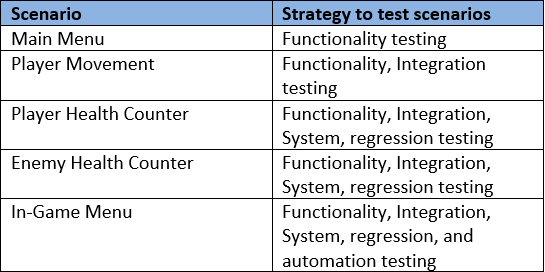
\includegraphics[scale=0.9]{./images/tactics.PNG}
\end{figure}

\newpage

\section{Testing Strategy}

\subsection{Unit Testing}
\subsubsection{Definition}
UNIT TESTING is a level of software testing where individual units/ components of a software are tested. The purpose is to validate that each unit of the software performs as designed.\cite{UT}
\subsubsection{Participants}
Developers
\subsubsection{Methodology}
Unit test case has been processed by Developers and they will write the test scripts for the unit testing if game.\cite{UT}
\begin{figure}[h!]
    \centering
    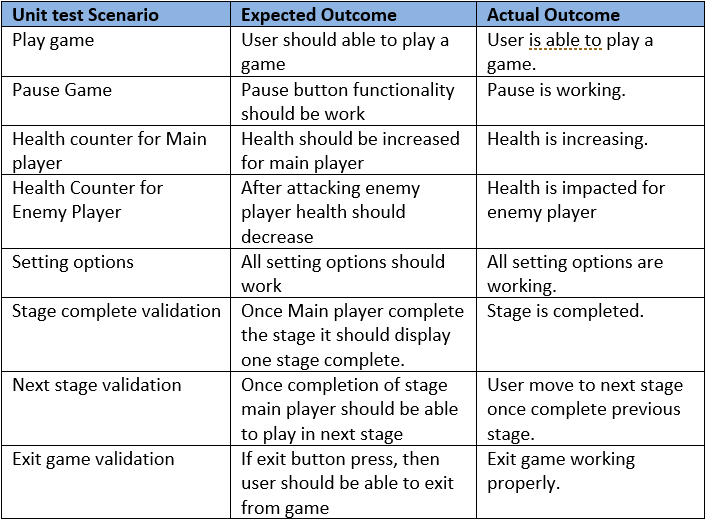
\includegraphics[scale=0.6]{./images/unittesting.PNG}
    \caption{Unit Testing}
    \label{fig:my_label}
\end{figure}

\newpage

\subsection{System and Integration Testing}
\subsubsection{Definition}
System Integration Testing is defined as a type of software testing carried out in an integrated hardware and software environment to verify the behaviour of the complete system. It is testing conducted on a complete, integrated system to evaluate the system's compliance with its specified requirement.
System Integration Testing (SIT) is performed to verify the interactions between the modules of a software system. It deals with the verification of the high and low-level software requirements specified in the Software Requirements Specification/Data and the Software Design Document.\cite{SIT}

\subsubsection{Participants}
Testing is performed using test data created by the testers.
\subsubsection{Methodology}
Once unit testing is completed then as a tester; they should test whole game from start to end with all the components from game. Tester will perform the testing and will create the test scripts.
\begin{figure}[h]
    \centering
    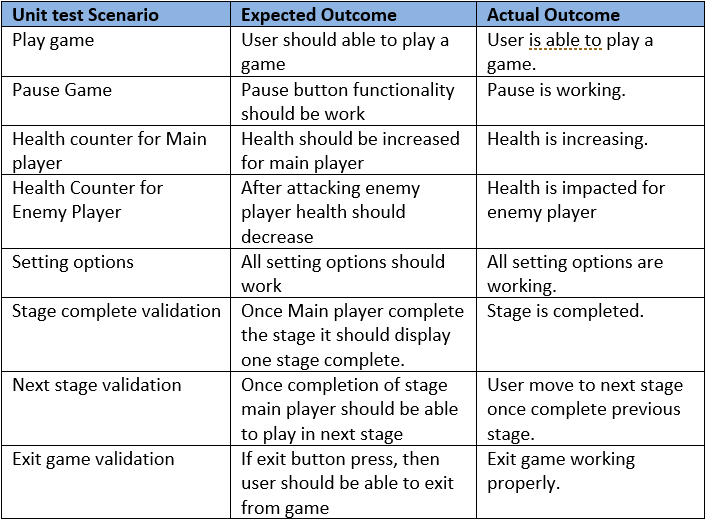
\includegraphics[scale=0.9]{./images/unittesting.PNG}
    \caption{System and Integration Testing}
    \label{fig:my_label}
\end{figure}
\subsection{Performance and Stress Testing}
\subsubsection{Definition}
PERFORMANCE TESTING checks the speed, response time, reliability, resource usage, scalability of a software program under their expected workload. The purpose of Performance Testing is not to find functional defects but to eliminate performance bottlenecks in the software or device.
STRESS TESTING is a type of Software Testing that verifies the stability & reliability of the system. This test mainly measures the system on its robustness and error handling capabilities under extremely heavy load conditions.\cite{ST}

\subsubsection{Participants}
Testers 
\subsubsection{Methodology}
For checking the game performance and at a time how many users can play a game we have to perform Stress and performance testing. Using Jmeter we can create n number of virtual users and check the performance of the game. Tester will create the test scripts.\cite{ST}
\begin{figure}[h]
    \centering
    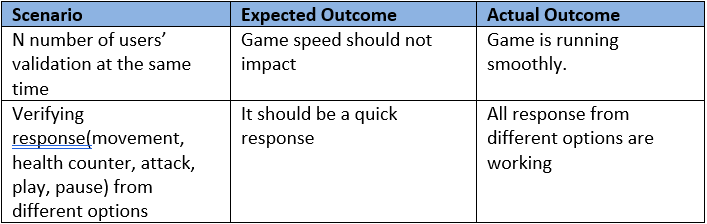
\includegraphics[scale=0.9]{./images/performanceAndStress.PNG}
    \caption{Performance and Stress Testing}
    \label{fig:my_label}
\end{figure}
\subsection{User Acceptance Testing }
\subsubsection{Definition}
User Acceptance Testing (UAT) is a type of testing performed by the end user or the client to verify/accept the software system before moving the software application to the production environment. UAT is done in the final phase of testing after functional, integration and system testing is done.\cite{AT}
\subsubsection{Participants}
End User OR Client
\subsubsection{Methodology}
To ensure a successful product delivery, we should follow 5 phase UAT process i.e. Planning, Coverage, Execution & Tracking, Reporting, and Reuse. As this has been executed by End user or client so tester will create either script or it can be executed manually.
\begin{figure}[h]
    \centering
    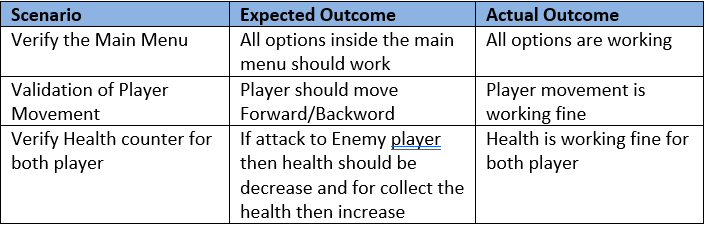
\includegraphics[scale=0.9]{./images/UserAcceptance.PNG}
    \caption{User Acceptance Testing}
    \label{fig:my_label}
\end{figure}
\subsection{Batch Testing}
\subsubsection{Definition}
Group of tests executing sequentially one by one is called Batch Testing.\cite{BT}
\subsubsection{Participants}
Testers 
\subsubsection{Methodology}
Batch testing can be conducted once we have all the test cases for the game. We will arrange all the test cases sequentially and will execute in a batch. For Example, if we have to test game like start  Pause  Resume then Exit. So we have to arrange all the test cases according to that and then we will execute all the test cases in Batch. Tester will create the scripts for batch execution.\cite{BT}

\subsection{Automated Regression Testing }
\subsubsection{Definition}
Regression tests ensure that code that was previously functioning correctly does not regress when changes are made. Having a comprehensive suite of unit level regression tests provides a safety net, making sure that code changes do not break existing functionality.\cite{RT} 
\subsubsection{Participants}
Tester and Developer
\subsubsection{Methodology}
Regression testing ensures that recent changes to the code leave the rest of the code intact, thereby preventing software regression. For Example, In Game If Main Player attack Enemy Player then Health should be impacted for enemy player. If main player health is less and if he/she picked health, then life should be increased. So if we are testing these scenario then it should work properly.\cite{RT}

\subsection{Beta Testing Participants}
\subsubsection{Participants}
End Users/Real Users
\subsubsection{Methodology}
\begin{itemize}
    \item All the components of the Game are ready to start this testing.
    \item Documentation that must reach the end users should be kept ready – Setup, Installation, Usage, Uninstallation should be detailed out and reviewed for correctness.
    \item Product Management team should review if each key functionality is in good working condition.
    \item Procedure to collect Bugs, feedback etc should be identified and reviewed to publish.
\end{itemize}

\newpage

\section{Testing Schedule}
\begin{figure}[h]
    \centering
    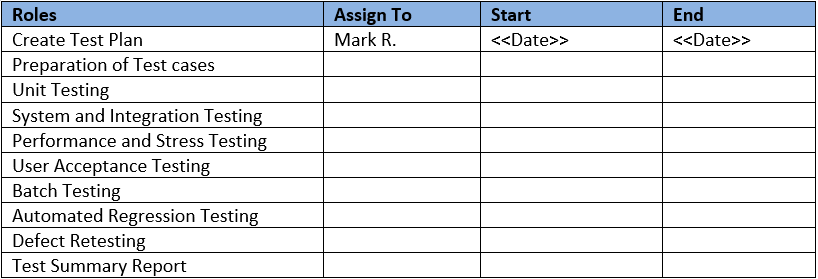
\includegraphics[scale=0.9]{./images/TestSchedule.PNG}
    \caption{Test Schedule}
    \label{fig:my_label}
\end{figure}
\textbf{Tools:}
\begin{figure}[h]
    \centering
    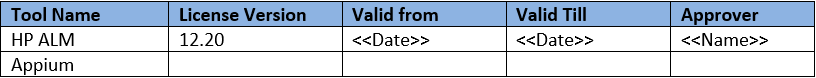
\includegraphics[scale=0.9]{./images/Tools.PNG}
    \caption{Tools}
    \label{fig:my_label}
\end{figure}

\textbf{Facilities:}
\begin{figure}[h]
    \centering
    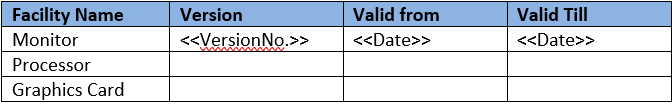
\includegraphics[scale=0.9]{./images/Facilities.PNG}
    \caption{Facilities}
    \label{fig:my_label}
\end{figure}
\newpage

\section{Control Procedures}
\subsection{Problem Reporting}
Any defect during game testing will be reported in below manner.
\begin{figure}[h]
    \centering
    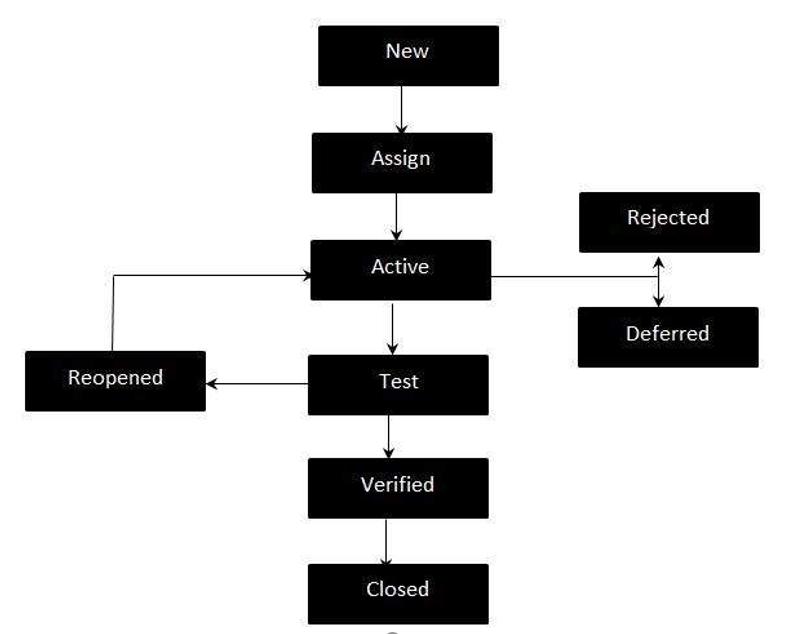
\includegraphics[scale=0.9]{./images/ControlProcedure.PNG}
    \caption{Control Procedure}
    \label{fig:my_label}
\end{figure}
\newpage

\subsection{Change Requests}
Below is the steps for change requests.
\begin{figure}[h]
    \centering
    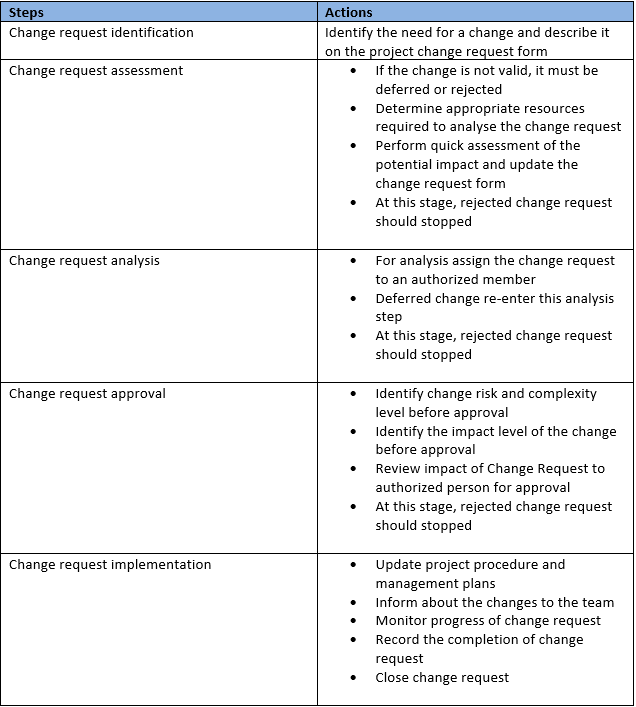
\includegraphics[scale=0.9]{./images/StepsControl.PNG}
    \caption{Change Requests}
    \label{fig:my_label}
\end{figure}
\newpage

\section{Features to be Tested}
Below is the list of features which will be tested as part of this release:

\begin{itemize}
    \item Background 
    \item Character Moving forward and Backwards
    \item Character Jump/Attack
    \item Game Pause/Play
    \item Selection of Player/Enemy Character
    \item Player/Enemy Projectile
    \item Ground Asset
    \item Health Pickup
    \item Rock Asset
    \item Menu Options (Play, Load, Delete Games)
    \item Settings
    \item Exit Game
    
\end{itemize}

\newpage

\section{Features not to be Tested}
\begin{itemize}
    \item Hardware Performance
    \item Installation of any packages
    \item Network performance 
    \item Server response
    \item Processors and memory constraints
\end{itemize}
\newpage

\section{Roles & Responsibilities}
\begin{itemize}
    \item Game producers are responsible for setting testing deadlines in coordination with marketing and quality assurance.They also manage many items outside of game testing, relating to the overall production of a title. Their approval is typically required for final submission.
    \item Lead tester, test lead or QA lead is the person responsible for the game working correctly and managing bug lists. A lead tester manages the QA staff. Lead tester works closely with designers and programmers, especially towards the end of the project. The lead tester is responsible for tracking bug reports and managing that they are fixed. They are also responsible that QA teams produce formal and complete reports.
    \item Testers are responsible for checking that the game works, is easy to use, has actions that make sense, and contains fun game play. Testers need to write accurate and specific bug reports, and if possible providing descriptions of how the bug can be reproduced. Testers may be assigned to a single game during its entire production, or brought onto other projects as demanded by the department's schedule and specific needs.
\end{itemize}
\begin{figure}[h]
    \centering
    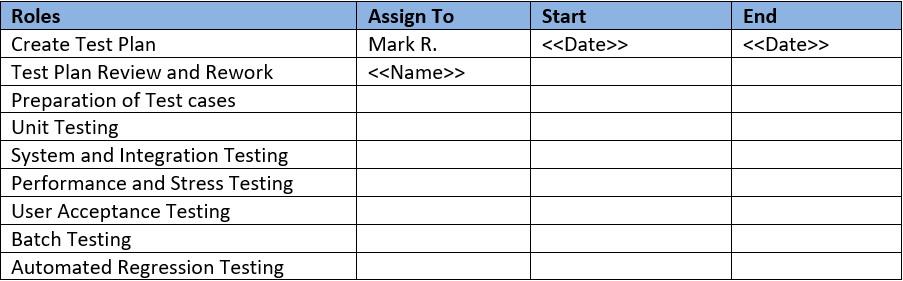
\includegraphics[scale=0.9]{./images/Roles.PNG}
    \caption{Roles}
    \label{fig:my_label}
\end{figure}

\newpage

\section{Schedules}
The following table highlights the tasks that will be carried out during this level of testing. These dates are accurate at the time of writing this document but can change as the project progresses.
\begin{figure}[h]
    \centering
    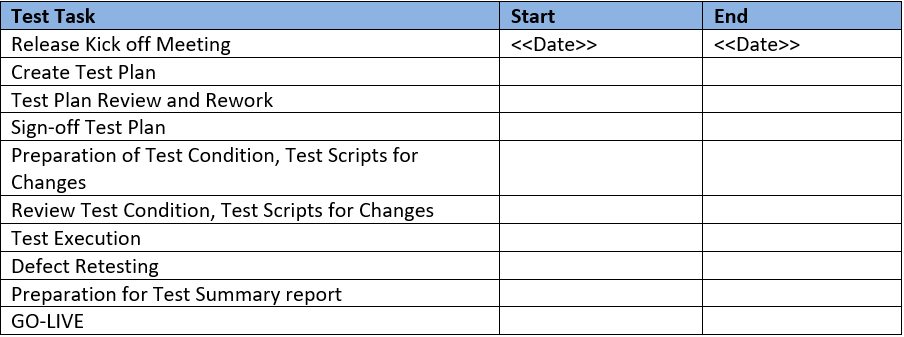
\includegraphics[scale=0.9]{./images/Schedule.PNG}
    \caption{Schedule}
    \label{fig:my_label}
\end{figure}

\newpage

\section{Dependencies, Issues, Risks and Assumptions}
\subsection{Dependencies}
The table below describes the dependencies related to system testing for this project:
\begin{figure}[h]
    \centering
    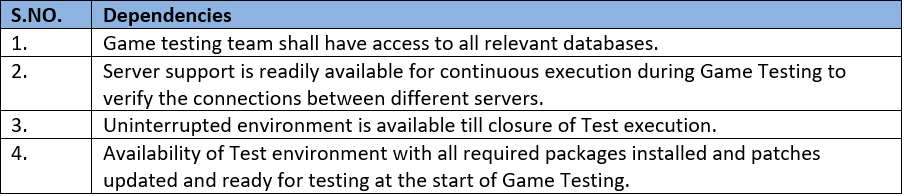
\includegraphics[scale=0.9]{./images/Dependencies.PNG}
    \caption{Dependencies}
    \label{fig:my_label}
\end{figure}
\subsection{Issues:}
The table below describes the open issues related to Application testing for this project:
\begin{figure}[h]
    \centering
    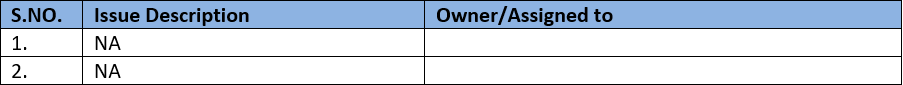
\includegraphics[scale=0.9]{./images/Issues.PNG}
    \caption{Issues}
    \label{fig:my_label}
\end{figure}

\subsection{Risks/Assumptions:}
The table below describes the assumptions related to testing:
\begin{figure}[h]
    \centering
    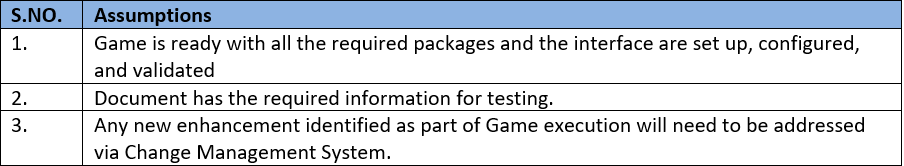
\includegraphics[scale=0.9]{./images/Assumptions.PNG}
    \caption{Assumptions}
    \label{fig:my_label}
\end{figure}

The table below describes the risks related to testing:
\begin{figure}[h]
    \centering
    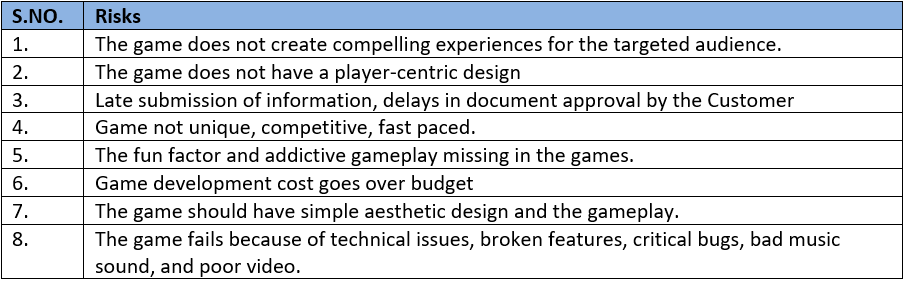
\includegraphics[scale=0.9]{./images/Risks.PNG}
    \caption{Risks}
    \label{fig:my_label}
\end{figure}
\newpage

\section{Tools}
Defect Management Tool – HP ALM (Application Lifecycle Management), JIRA, BUGZILLA
Automation Tool – APPIUM, MAuto 

\newpage

\printbibliography
\end{document}
